\begin{figure}[H]
\caption{Lambda Architecture}
\centering
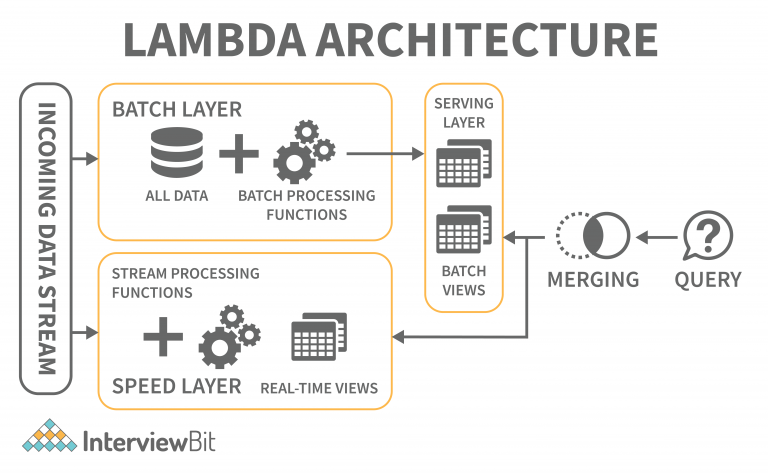
\includegraphics[width=1\linewidth]{images/Lambda-Architecture-768x475.png}
\small
\textit{Note.} The image depicts the Lambda architecture, a data processing framework designed for handling big data in real-time applications. \textbf{Batch Layer} — Processes all data and performs batch processing functions; \textbf{Speed Layer} — Handles stream processing and real-time views; \textbf{Serving Layer} — Provides batch views and merges data for queries; \textbf{Incoming Data Stream} — Feeds into both batch and speed layers; \textbf{Merging} — Combines batch and real-time processed data.
\textit{Creator.} (\cite{interviewBit})\footnote[39]{\fullcite{interviewBit}}
\end{figure}